\documentclass[tikz,border=6pt]{standalone}
\usetikzlibrary{arrows.meta}

\begin{document}
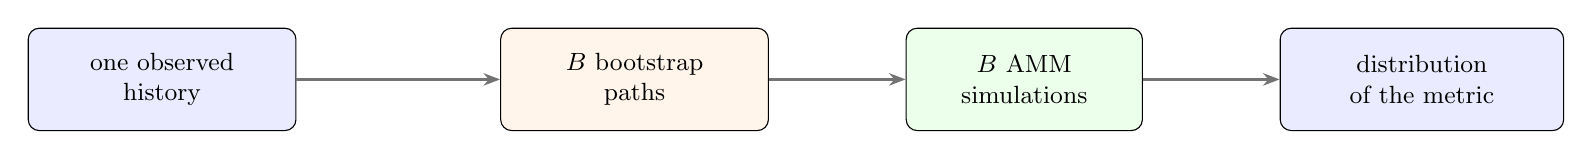
\begin{tikzpicture}[
    box/.style={draw, rounded corners, align=center, minimum height=1.3cm, inner sep=6pt, font=\small},
    arr/.style={-{Stealth[length=6pt]}, thick, black!55}
  ]

  \node[box, fill=blue!8, minimum width=3.4cm] (hist) at (0, 0) {one observed \\ history};
  \node[box, fill=orange!8, minimum width=3.4cm] (paths) at (6.0, 0) {$B$ bootstrap \\ paths};
  \node[box, fill=green!8, minimum width=3.0cm] (sim) at (10.95, 0) {$B$ AMM \\ simulations};
  \node[box, fill=blue!8, minimum width=3.6cm] (dist) at (16.0, 0) {distribution \\ of the metric};

  \draw[arr] (hist.east) -- (paths.west);
  \draw[arr] (paths.east) -- (sim.west);
  \draw[arr] (sim.east) -- (dist.west);

\end{tikzpicture}
\end{document}
